\documentclass[11pt]{article}
\usepackage[margin=1in]{geometry}
\usepackage[T1]{fontenc}
\usepackage{mathptmx}

\usepackage{amsmath,amssymb,amsthm}
\usepackage{booktabs}
\usepackage{graphicx}
\usepackage{listings}
\usepackage[hidelinks]{hyperref}

\newtheorem{theorem}{Theorem}[section]
\newtheorem{proposition}[theorem]{Proposition}
\newtheorem{lemma}[theorem]{Lemma}
\newtheorem{corollary}[theorem]{Corollary}
\theoremstyle{definition}
\newtheorem{definition}[theorem]{Definition}
\theoremstyle{remark}
\newtheorem{remark}[theorem]{Remark}

\newcommand{\R}{\mathbb{R}}
\newcommand{\nrm}[1]{\lVert #1\rVert}
\lstset{basicstyle=\ttfamily\small,frame=single,breaklines=true,columns=fullflexible}

\title{The Swarm Simulator:\\ A Dynamical Systems Model of Collective Intelligence\\
Using the TO/TOGT Operator Pipeline\\[4pt]
\large Version 3 --- corrections and formal checks}
\author{Pablo Nogueira Grossi\\ G6 LLC, Newark, New Jersey, USA\\
ORCID: 0009-0000-6496-2186}
\date{September 2026\\[2pt]
{\small V1: 10.5281/zenodo.19208284 \quad V2: 10.5281/zenodo.20230613 \quad V3: 10.5281/zenodo.23027566}}

\begin{document}
\maketitle

\begin{abstract}
We define the Swarm Simulator, a multi-agent dynamical system whose collective state
$X_t=(I_t,C_t,M_t,F_t)$ (shared-intent stability, coordination efficiency, type-propagation multiplier,
diffusion factor) evolves under four operators motivated by the TO/TOGT pipeline $G=U\circ F\circ K\circ C$.
Versions 1 and 2 stated a contraction theorem on $\R^4$ and a multi-orbit claim. Checking them against a
formal proof assistant (Lean~4.32.0, Mathlib v4.32.0) showed that the contraction theorem as printed is false:
the coordination update multiplies two state variables, so the map has no global Lipschitz constant.
This version proves the correct statements: contraction on a ball of explicit radius, geometric decay,
a unique fixed point at $0$ for $(I,C,M)$, and unbounded growth of $F$. It also shows that clusters satisfying
the contraction condition share that fixed point, so the multi-orbit claim of distinct fixed points does
not follow for this model. All theorems below are verified in Lean without \texttt{sorry}, using only the axioms
\texttt{propext}, \texttt{Classical.choice} and \texttt{Quot.sound}. Empirical calibration is not attempted.
\end{abstract}

\noindent\textbf{MSC:} 37C25, 37D10, 47H10, 68T99.\quad
\textbf{Note on preparation.} The corrections and the Lean checks in this version were prepared with Claude
(Anthropic). The model, the claims and the deposit are the author's.

\section{Relation to Prior Work}
The mathematical study of multi-agent dynamical systems has produced rigorous models of flocking, consensus
and emergent collective behaviour. Cucker and Smale~\cite{cs} and Olfati-Saber~\cite{os} established convergence
guarantees for distributed agents with local rules. More recent formulations include overdamped Langevin
models for swarm cooperation~\cite{nitti} and minimal systems exhibiting flocking and swarming
together~\cite{sar}. Contraction theory is a standard tool for global convergence in multi-agent
systems~\cite{riv}, and Leonard~\cite{leo} surveys the bifurcation structures of collective migration and
decision making, including pitchfork bifurcations in honeybee-inspired models~\cite{gray}.

The present model is not a physical or biological model. It is an operator-algebraic construction whose four
collective operators are taken here as definitions. The agent-level pipeline $G=U\circ F\circ K\circ C$ of
TO/TOGT motivates them but is not formalised in this paper.

\section{Swarm State Space}
\begin{definition}[Swarm state]
The swarm state at time $t$ is $X_t=(I_t,C_t,M_t,F_t)$: $I_t$ shared-intent stability, $C_t$ coordination
efficiency, $M_t$ type-propagation multiplier, $F_t$ diffusion factor.
\end{definition}

\section{Collective Operators}
\begin{definition}[Definitions 3.1--3.4]\label{def:ops}
\begin{align*}
I_{t+1} &= I_t\cdot f_{\rm types}\cdot f_{\rm agents}\cdot(1-\eta),\\
C_{t+1} &= C_t\cdot I_{t+1}\cdot \frac{1}{1+D},\\
M_{t+1} &= M_t\,(1+\beta\cdot{\rm reuse})\cdot \overline{q},\\
F_{t+1} &= 1+\alpha t.
\end{align*}
\end{definition}
Write
\[
a=f_{\rm types}f_{\rm agents}(1-\eta),\qquad c=\frac1{1+D},\qquad m=(1+\beta\,{\rm reuse})\,\overline q,
\]
all assumed non-negative. For $X=(I,C,M)\in\R^3$ put $\nrm X=|I|+|C|+|M|$ and
\[
G(X)=\bigl(aI,\; C\,(aI)\,c,\; mM\bigr).
\]
The coordinate $F_t=1+\alpha t$ depends on $t$ and not on the state, so $G$ is defined on $(I,C,M)$ and
$F$ is treated separately (Proposition~\ref{prop:F}). The composite operator of V1,
$G_{\rm swarm}=F\circ M\circ C\circ I$, is $G$ together with the update of $F$.

\section{Dynamics: what holds and what does not}
In V1 the constants $L_I=a$, $L_C=a/(1+D)$, $L_M=m$ and $L=L_I+L_C+L_M$ were introduced, and the paper stated
that $L<1$ makes $G_{\rm swarm}$ a contraction on $\R^4$ with the $\ell^1$ norm, with a unique fixed point and
the bound $\nrm{X_t-X^*}\le L^t\nrm{X_0-X^*}$. The first statement is false. What is true is below.

\begin{proposition}[No global Lipschitz constant]\label{prop:nolip}
If $a>0$ and $c>0$, then for every $K$ there are $X,Y\in\R^3$ with $\nrm{G(X)-G(Y)}>K\nrm{X-Y}$.
\end{proposition}
\begin{proof}
Take $X=(1,C_0,0)$ and $Y=(0,C_0,0)$ with $C_0=(|K|+1)/(ac)$. Then $\nrm{X-Y}=1$, $G(Y)=0$ and
$G(X)=(a,\,C_0ac,\,0)=(a,\,|K|+1,\,0)$, so $\nrm{G(X)-G(Y)}=a+|K|+1>K$.
\end{proof}

\begin{theorem}[Contraction on a ball]\label{thm:ball}
Let $X,Y\in\R^3$ with $|C_X|\le R$ and $|I_Y|\le R$. Then
\[
\nrm{G(X)-G(Y)}\le\lambda(R)\,\nrm{X-Y},\qquad \lambda(R)=\max\{a(1+cR),\,m\}.
\]
If $a<1$ and $m<1$, then $\lambda(R)<1$ exactly when $R<(1-a)/(ac)$.
\end{theorem}
\begin{proof}
The three coordinates of $G(X)-G(Y)$ are $a\Delta I$, $ac\,(C_XI_X-C_YI_Y)$ and $m\Delta M$. Since
$C_XI_X-C_YI_Y=C_X\Delta I+I_Y\Delta C$, the middle one has modulus at most $acR(|\Delta I|+|\Delta C|)$. Summing,
$\nrm{G(X)-G(Y)}\le(a+acR)|\Delta I|+acR|\Delta C|+m|\Delta M|\le\lambda(R)\nrm{X-Y}$, because $acR\le a(1+cR)$.
\end{proof}

For $R\ge0$ put $\rho(R)=\max\{a,\;acR,\;m\}$.

\begin{lemma}\label{lem:size}
If $\nrm X\le R$ then $\nrm{G(X)}\le\rho(R)\,\nrm X$.
\end{lemma}
\begin{proof}
$|I|\le R$, so $|C'|=ac|I||C|\le acR|C|$; hence $\nrm{G(X)}=a|I|+ac|I||C|+m|M|\le\rho(R)\nrm X$.
\end{proof}

\begin{theorem}[Fixed point]\label{thm:fixed}
$G(0)=0$. If $\rho(R)<1$ and $\nrm X\le R$ with $G(X)=X$, then $X=0$.
\end{theorem}
\begin{proof}
By Lemma~\ref{lem:size}, $\nrm X=\nrm{G(X)}\le\rho(R)\nrm X$, so $(1-\rho(R))\nrm X\le0$.
\end{proof}

\begin{theorem}[Decay]\label{thm:decay}
If $\rho(R)\le1$ and $\nrm{X_0}\le R$, then $\nrm{X_t}\le\rho(R)^t\nrm{X_0}$ for all $t\ge0$. If moreover
$L=a+\frac{a}{1+D}+m<1$ and $\nrm{X_0}\le1$, then
\[
\nrm{X_t}\le L^t\nrm{X_0}\qquad(t\ge0).
\]
\end{theorem}
\begin{proof}
Induction with Lemma~\ref{lem:size}: $\nrm{X_t}\le\nrm{X_0}\le R$ keeps the orbit in the ball. For the second
statement take $R=1$ and note $\rho(1)=\max\{a,ac,m\}\le a+ac+m=L$.
\end{proof}

\begin{remark}[The printed bound fails from large starts]\label{rem:fail}
For the default parameters $f_{\rm types}=0.65$, $f_{\rm agents}=0.80$, $\eta=0.20$, $D=1.5$, $\beta=0.10$,
${\rm reuse}=0.50$, $\overline q=0.22$ we have exactly $a=52/125$, $c=2/5$, $m=231/1000$, so $L=0.8134<1$. The
ball condition of Theorem~\ref{thm:ball} holds for $R<365/104\approx3.51$. From $X_0=(100,10,1)$ one step gives
$G(X_0)=(41.6,\,166.4,\,0.231)$ with $\nrm{G(X_0)}=208.231>L\cdot111=90.2874$, and the bound fails at each of
the steps $t=1,\dots,5$. With seed 2026, starts drawn from $[0,3]^3$ never violate the printed bound, from $[0,10]^3$ about $3\%$ do, and
from $[0,100]^3$ about $88\%$ do.
\end{remark}

\begin{remark}[Shared intent is a chain]
$I_t=a^tI_0$ exactly, with $a=0.416$ for the default parameters: $I_{10}=1.55\times10^{-4}I_0$ and
$I_{20}=2.41\times10^{-8}I_0$. This is the law that a chain of $t$ steps, each holding with probability $a$,
holds with probability $a^t$. In this model shared intent, coordination and type propagation all decay to $0$.
\end{remark}

\begin{proposition}[The diffusion coordinate]\label{prop:F}
If $\alpha>0$, then $F_t=1+\alpha t$ has no upper bound. The four-coordinate system therefore has no fixed
point, and the theorems above concern $(I,C,M)$.
\end{proposition}

\section{Multi-Orbit Systems}
V1 stated that when several clusters each satisfy the contraction condition, the swarm forms a multi-orbit
system $S=\{O_1,\dots,O_k\}$ whose orbits converge to distinct fixed points, with $\mathrm{Inv}(S)\supsetneq\bigcup_i\mathrm{Inv}(O_i)$.

\begin{proposition}\label{prop:two}
Let clusters $i=1,2$ have constants $(a_i,c_i,m_i)$ with $\rho_i(R)<1$. Any fixed points $X_1,X_2$ of the two
maps in the ball $\nrm X\le R$ are equal to $0$. In particular the two clusters have the same fixed point and
differ only in their decay rates.
\end{proposition}
\begin{proof}
Theorem~\ref{thm:fixed} for each cluster.
\end{proof}

The V2 simulation of two clusters converging to ``distinct fixed points'' used parameter sets with printed
$L=2.41$ and $L=1.93$, so neither satisfied the contraction condition, and both runs converged to $0$
numerically. The inclusion $\mathrm{Inv}(S)\supsetneq\bigcup\mathrm{Inv}(O_i)$ of V2 (its theorem T9) holds by
construction, because the system invariant was defined as the maximum of the orbit invariants plus one, and it
carries no information about the dynamics. Distinct fixed points would require a model with a persistent source,
for example an inflow term in $I$; none is proposed here.

\section{Minimal Simulator}
\begin{lstlisting}[language=Python]
def step(state, p, t):
    I, C, M, F = state
    I_new = I * p.type_quality * p.agent_quality * (1 - p.noise)
    C_new = C * I_new / (1 + p.drag)
    M_new = M * (1 + p.beta * p.reuse) * p.avg_quality
    F_new = 1 + p.alpha * t
    return (I_new, C_new, M_new, F_new)
\end{lstlisting}
The full simulator, with \texttt{python swarm\_simulator.py --check} (ten numerical checks of the statements
proved in Lean), is in the deposit. Figures~\ref{fig:evo}--\ref{fig:two} are its output.

\begin{figure}[ht]\centering
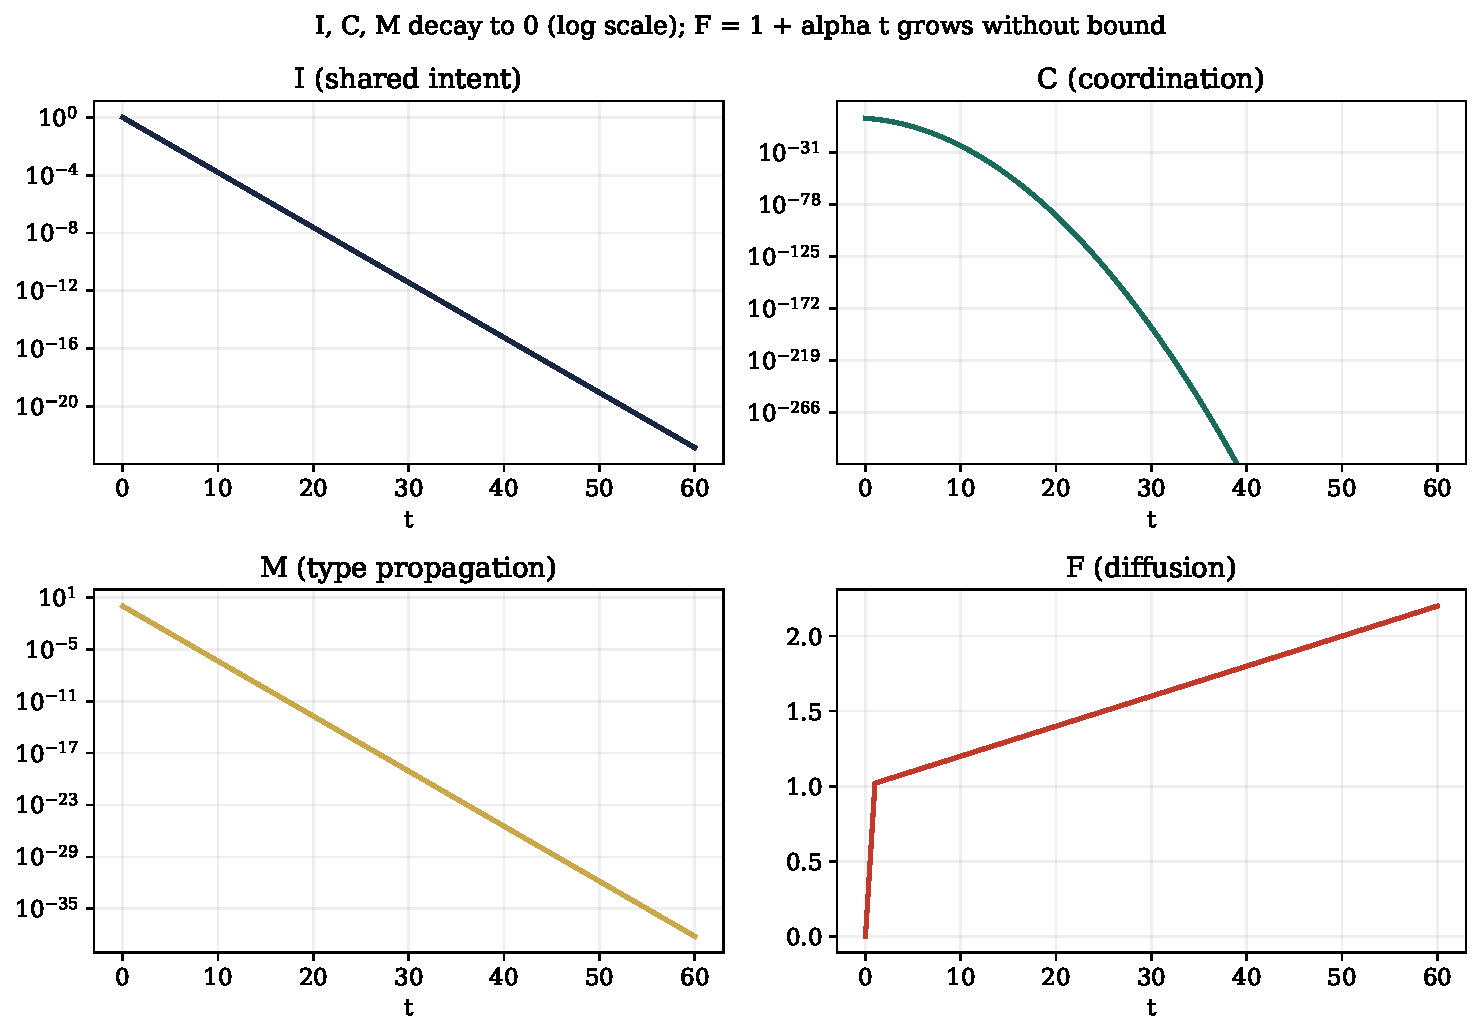
\includegraphics[width=0.78\textwidth]{figures/fig1_state_evolution.pdf}
\caption{$I$, $C$, $M$ decay to $0$ (logarithmic scale) and $F=1+\alpha t$ grows without bound.}\label{fig:evo}
\end{figure}
\begin{figure}[ht]\centering
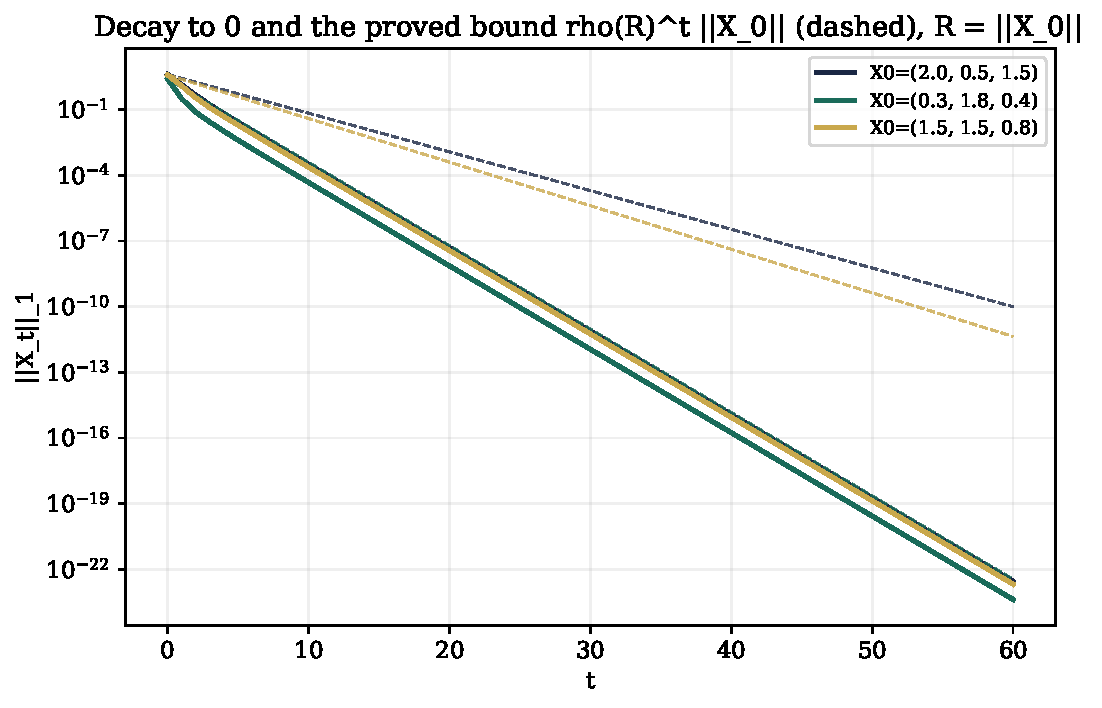
\includegraphics[width=0.66\textwidth]{figures/fig2_convergence.pdf}
\caption{Three starting states and the proved bound $\rho(R)^t\nrm{X_0}$ with $R=\nrm{X_0}$ (dashed).}\label{fig:conv}
\end{figure}
\begin{figure}[ht]\centering
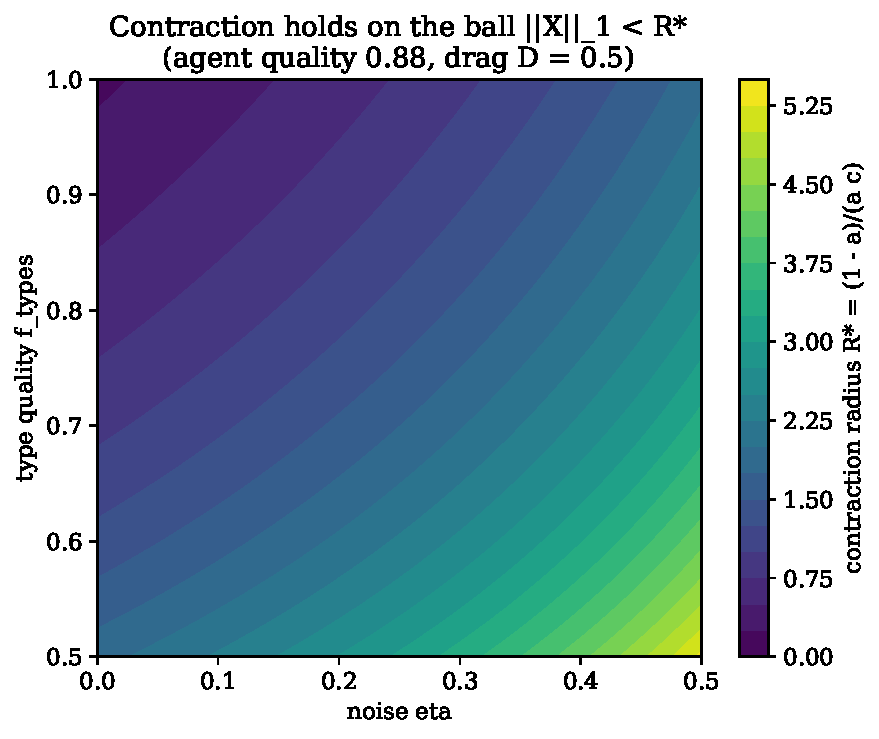
\includegraphics[width=0.52\textwidth]{figures/fig3_contraction_region.pdf}
\caption{Contraction radius $R^*=(1-a)/(ac)$ over noise and type quality (agent quality $0.88$, $D=0.5$).}\label{fig:region}
\end{figure}
\begin{figure}[ht]\centering
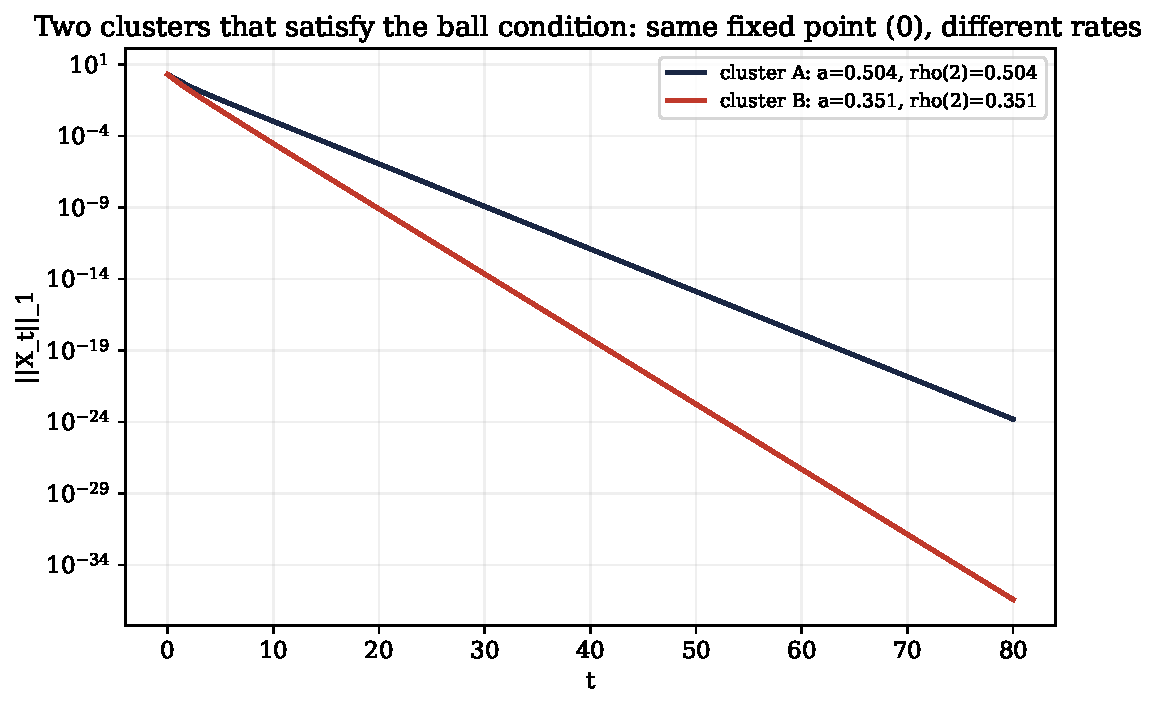
\includegraphics[width=0.66\textwidth]{figures/fig4_multi_orbit.pdf}
\caption{Two clusters that satisfy the ball condition: the same fixed point, different decay rates.}\label{fig:two}
\end{figure}

\section{Formal Verification}
The file \texttt{SwarmSimulator.lean} (V3) compiles with Lean~4.32.0 and Mathlib v4.32.0 with no \texttt{sorry}.
The \texttt{\#print axioms} report lists only \texttt{propext}, \texttt{Classical.choice}, \texttt{Quot.sound}
for each theorem in Table~\ref{tab:lean}. The file was compiled in a cloud environment; the author's audit run is
recorded in the deposit.
\begin{table}[ht]\centering\small
\begin{tabular}{@{}ll@{}}\toprule
Lean theorem & Statement\\\midrule
\texttt{no\_global\_lipschitz} & Proposition~\ref{prop:nolip}\\
\texttt{step\_lipschitz\_ball} & Theorem~\ref{thm:ball}\\
\texttt{fixed\_point\_zero}, \texttt{step\_zero} & Theorem~\ref{thm:fixed}\\
\texttt{orbit\_nrm\_le}, \texttt{paper\_bound} & Theorem~\ref{thm:decay}\\
\texttt{printed\_bound\_fails} & the first step of Remark~\ref{rem:fail}, in exact arithmetic\\
\texttt{default\_radius} & $a(1+\tfrac25\cdot\tfrac72)<1<a(1+\tfrac25\cdot4)$ for $a=52/125$\\
\texttt{two\_clusters} & Proposition~\ref{prop:two}\\
\texttt{diffuse\_unbounded} & Proposition~\ref{prop:F}\\\bottomrule
\end{tabular}
\caption{Fourteen theorems in the file, of which these are the ones the paper uses (the rest are lemmas).}\label{tab:lean}
\end{table}

\section{Open Questions}
\begin{description}
\item[S3 (calibration).] The default parameters are not fitted to data. Calibration against, for example,
Sinhuber et al.\ (2019) or Nitti et al.~\cite{nitti} has not been attempted. A calibration would also have to
account for shared intent that persists, which this model does not produce.
\item[Persistent state.] Whether a model in this family with a source term has distinct, non-zero fixed
points for different clusters is not addressed.
\item[Agent level.] The agent-level pipeline $G=U\circ F\circ K\circ C$ is not formalised here.
\end{description}

\section{Corrections since V1}
V1 (March 2026) stated Theorems 5.1--5.3 and the multi-orbit claim without proof, as following from earlier
results of the series, and described the paper as making no numerical claims. V2 (May 2026) added a Python
simulator and a Lean file. In V3: (i) Theorem 5.1 as printed is replaced by Theorem~\ref{thm:ball}, because it is
false as stated (Proposition~\ref{prop:nolip}); (ii) the printed convergence bound is replaced by
Theorem~\ref{thm:decay}, and its failure is recorded (Remark~\ref{rem:fail}); (iii) the multi-orbit claim is
replaced by Proposition~\ref{prop:two}; (iv) the V2 Lean file, which did not compile on the pinned toolchain, is
replaced; (v) the simulator's fixed-point routine and its figures are corrected.

\begin{thebibliography}{9}
\bibitem{nitti} A.~Nitti, I.~Federico, M.~D.~de Tullio, G.~Carbone. A collective intelligence model for swarm robotics applications. \emph{Nature Communications} 16:6572, 2025.
\bibitem{sar} G.~K.~Sar, D.~Ghosh. Flocking and swarming in a multi-agent dynamical system. \emph{Chaos} 33(12):123126, 2023.
\bibitem{riv} P.~M.~Rivera-Ortiz, A.~C.~Frommer, Y.~Diaz-Mercado. Contraction analysis of multi-agent control for guaranteed capture of a faster evader. \emph{ASME Letters in Dynamic Systems and Control} 4(3):031001, 2024.
\bibitem{leo} N.~E.~Leonard. Multi-agent system dynamics: Bifurcation and behavior of animal groups. \emph{Annual Reviews in Control} 38(1):1--14, 2014.
\bibitem{os} R.~Olfati-Saber. Flocking for multi-agent dynamic systems: Algorithms and theory. \emph{IEEE Trans.\ Automatic Control} 51(3):401--420, 2006.
\bibitem{cs} F.~Cucker, S.~Smale. Emergent behavior in flocks. \emph{IEEE Trans.\ Automatic Control} 52(5):852--862, 2007.
\bibitem{gray} R.~Gray, M.~Frasca, N.~E.~Leonard, et al. Multi-agent decision-making dynamics inspired by honeybees. \emph{IEEE Trans.\ Control of Network Systems} 5(4):1576--1586, 2018.
\end{thebibliography}

\end{document}
